\item \textbf{{[}ALVL/9597/2017/P2/Q2{]} }

A multinational company has many local branches in various parts of
the country that are linked using a wide area network (WAN). 
\begin{enumerate}
\item The company's network transfers data using asynchronous data transmission. 
\begin{enumerate}
\item State which of the following diagrams represents asynchronous data
transmission. Explain your answer. \hfill{}{[}2{]}
\begin{center}
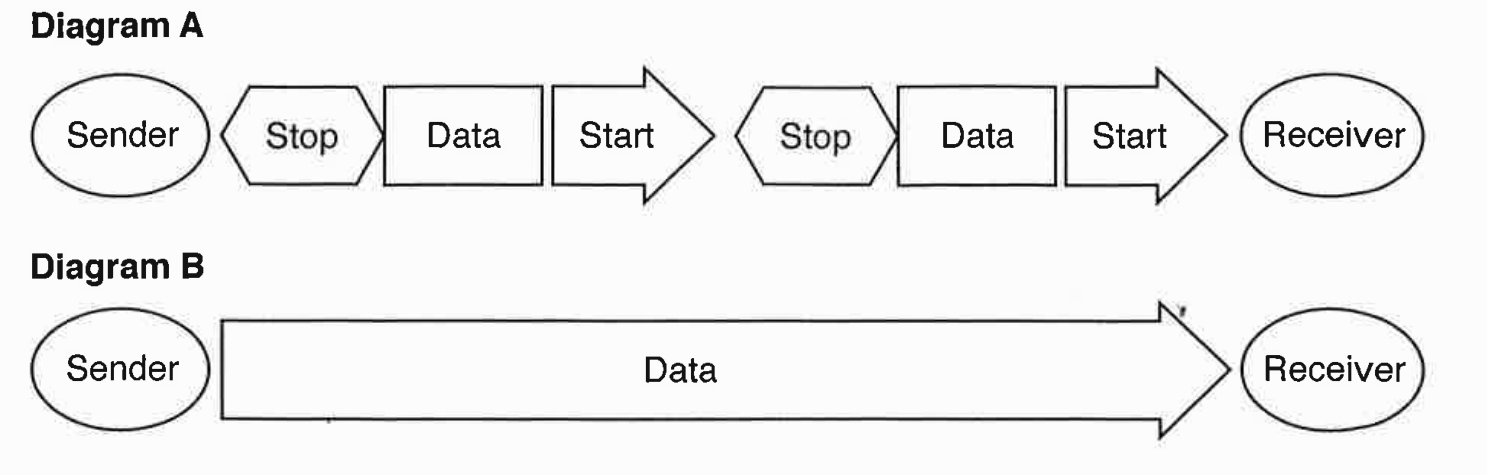
\includegraphics[width=0.5\paperwidth]{C:/Users/Admin/Desktop/Github/question_bank/LyX/static/img/9597-ALVL-2017-P2-Q2-1}
\par\end{center}
\item Explain why asynchronous data transmission affects network performance.\hfill{}
{[}2{]}
\end{enumerate}
\end{enumerate}
An employee works from home on her wireless laptop. The following
diagram shows the configuration of the employee's home network.
\begin{center}
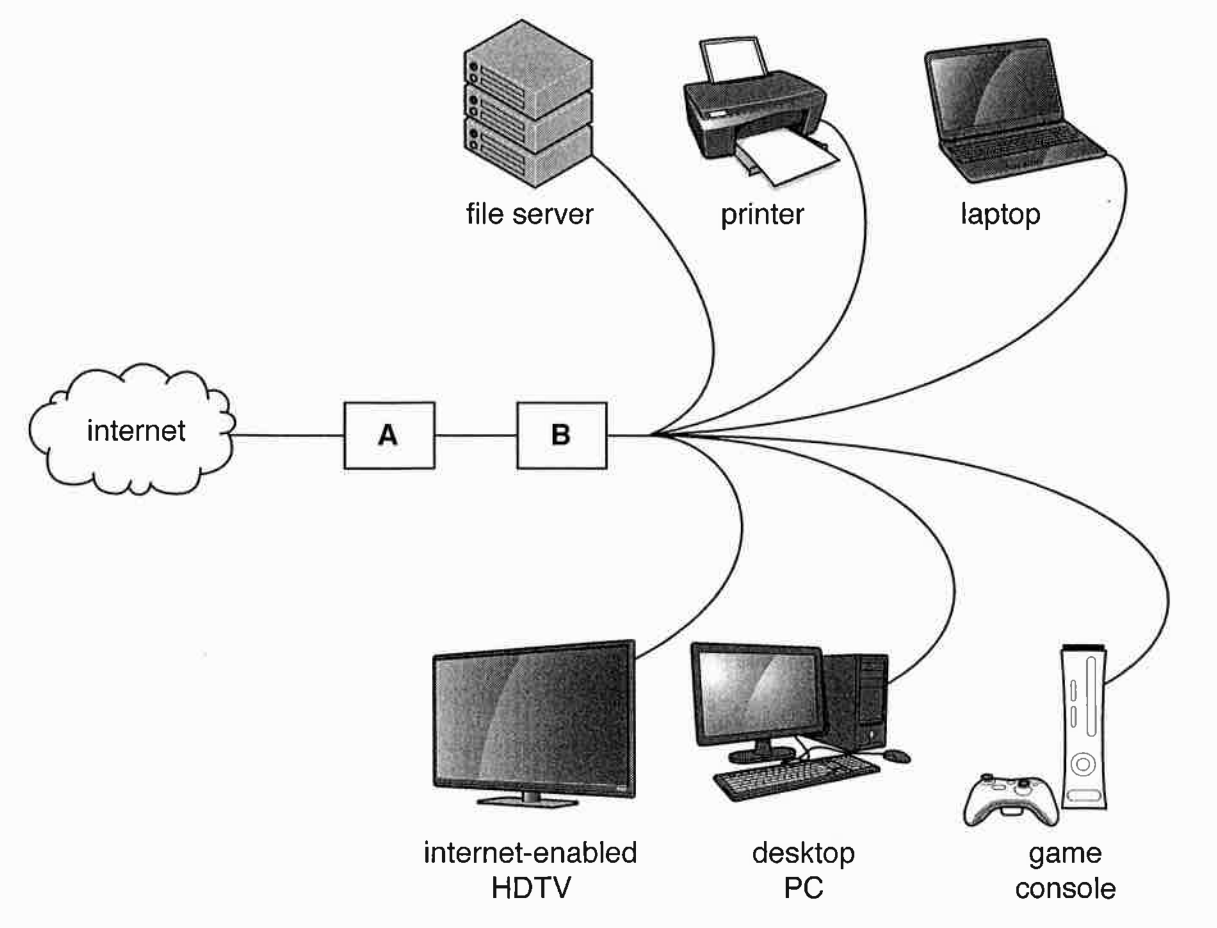
\includegraphics[width=0.5\paperwidth]{C:/Users/Admin/Desktop/Github/question_bank/LyX/static/img/9597-ALVL-2017-P2-Q2-2}
\par\end{center}
\begin{enumerate}
\item[(b)] This network uses both a switch and a router to transfer data. State
which of the pieces of equipment labelled \textbf{A} and \textbf{B}
is the switch. Explain your answer. \hfill{}{[}2{]}
\item[(c)] Describe \textbf{two} features of a router.\hfill{} {[}2{]}
\item[(d)] Describe \textbf{one} advantage and \textbf{one} disadvantage. for
the employee, of working from home.\hfill{} {[}2{]}
\end{enumerate}